\documentclass[11pt,a4paper]{article}

% Configuración de página y márgenes
\usepackage[margin=1in, top=1.2in, bottom=1.2in]{geometry}

% Configuración para manejar líneas largas y overflow
\sloppy
\emergencystretch=1em

% Paquetes para caracteres especiales y codificación
\usepackage[utf8]{inputenc}
\usepackage[T1]{fontenc}
\usepackage{lmodern}
\usepackage{textcomp}
\usepackage{amsmath}
\usepackage{amssymb}
\usepackage{gensymb}

% Soporte para idiomas (español e inglés)
\usepackage[spanish,english]{babel}

% Paquetes para imágenes y gráficos
\usepackage{graphicx}
\usepackage{float}
\usepackage{caption}
\usepackage{subcaption}

% Paquetes para tablas
\usepackage{longtable}
\usepackage{booktabs}
\usepackage{array}
\usepackage{multirow}
\usepackage{multicol}
\usepackage{tabularx}

% Paquetes para listas mejoradas
\usepackage{enumitem}

% Control de saltos de página
\usepackage{needspace}
\usepackage{afterpage}
\usepackage{placeins}

% Enlaces e hipervínculos
\usepackage[colorlinks=true, linkcolor=blue, urlcolor=blue, citecolor=blue]{hyperref}

% Paquetes para código y verbatim
\usepackage{fancyvrb}
\usepackage{listings}
\usepackage{xcolor}

% Paquetes para diseño profesional
\usepackage{tcolorbox}
\usepackage{tikz}
\tcbuselibrary{most}
\usepackage{fancyhdr}
\usepackage{lastpage}

% Configuración de encabezados y pies de página
\pagestyle{fancy}
\fancyhf{} % Limpiar encabezados y pies

% Pie de página
\fancyfoot[L]{\small UNIT Electronics - Development}
\fancyfoot[C]{\small July 2025}
\fancyfoot[R]{\small Page \thepage\ of \pageref{LastPage}}

% Línea en encabezado y pie
\renewcommand{\headrulewidth}{0.4pt}
\renewcommand{\footrulewidth}{0.4pt}

% Estilo para primera página de cada sección
\fancypagestyle{plain}{
    \fancyhf{}
    \fancyfoot[L]{\small UNIT Electronics - Development}
    \fancyfoot[C]{\small July 2025}
    \fancyfoot[R]{\small Page \thepage\ of \pageref{LastPage}}
    \renewcommand{\headrulewidth}{0pt}
    \renewcommand{\footrulewidth}{0.4pt}
}

% Configuración de listings para código
\lstset{
    basicstyle=\ttfamily\scriptsize,
    breaklines=true,
    frame=single,
    backgroundcolor=\color{gray!10},
    keywordstyle=\color{blue},
    commentstyle=\color{green!50!black},
    stringstyle=\color{red},
    showstringspaces=false,
    tabsize=2,
    breakatwhitespace=true,
    columns=flexible
}

% Configuración adicional para verbatim con líneas largas
\usepackage{alltt}
\renewcommand{\ttdefault}{pcr}

% Paquetes para mejor tipografía
\usepackage{microtype}
\usepackage{setspace}

% Configuración de espaciado
\onehalfspacing

% Configuración de listas anidadas
\setlist[itemize]{nosep, leftmargin=*, before=\vspace{0.5\baselineskip}, after=\vspace{0.5\baselineskip}}
\setlist[itemize,1]{label=\textbullet}
\setlist[itemize,2]{label=\textendash}
\setlist[itemize,3]{label=\textasteriskcentered}
\setlist[enumerate]{nosep, leftmargin=*, before=\vspace{0.5\baselineskip}, after=\vspace{0.5\baselineskip}}

% Comandos personalizados
\providecommand{\tightlist}{}

% Comando para evitar viudas y huérfanas
\widowpenalty=10000
\clubpenalty=10000

% Configuración de profundidad de numeración - sin numeración automática para secciones principales
\setcounter{secnumdepth}{2}
\setcounter{tocdepth}{3}

\begin{document}


% Página de título estandarizada IEEE/ISO
\begin{titlepage}
    \centering
    
    % Header corporativo estandarizado
    \vspace*{0.5cm}
    
    % Logo y información corporativa
    \begin{minipage}{0.3\textwidth}
        \centering
        
        
\includegraphics[width=\textwidth]{logo.png}
        
    \end{minipage}
    \hfill
    \begin{minipage}{0.6\textwidth}
        \raggedleft
        {\small \textbf{UNIT Electronics}}\\
        {\footnotesize Technical Documentation}\\
        {\footnotesize Development Project - Prototype Phase}
    \end{minipage}
    
    \vspace{2cm}
    
    % Título principal
    {\huge \textbf{Electronic Module}}\\[0.5cm]
    
    % Subtítulo
    
    {\Large Technical Datasheet and Development Guide}\\[1cm]
    
    
    % Información del producto
    
    {\large \textbf{Product:} Electronic Module}\\[0.3cm]
    
    
    
    {\large \textbf{SKU:} UEXXXX}\\[0.3cm]
    
    
    
    {\large \textbf{Version:} 1.0.0}\\[1cm]
    
    
    \vfill
    
    % Información de fechas y estado
    \begin{minipage}{0.45\textwidth}
        \centering
        \textbf{Project Phase}\\
        Prototype Development
    \end{minipage}
    \hfill
    \begin{minipage}{0.45\textwidth}
        \centering
        \textbf{Hardware Status}\\
        Functional prototype completed
    \end{minipage}
    
    \vspace{1cm}
    
    % Pie de página con fecha y copyright
    {\large July 2025}\\[0.5cm]
    {\footnotesize © 2025 UNIT Electronics. All rights reserved.}
    
\end{titlepage}

% Página de información técnica
\newpage
\thispagestyle{plain}

\section*{Document Information}

\begin{table}[H]
\centering
\begin{tabular}{ll}
\toprule
\textbf{Field} & \textbf{Value} \\
\midrule
Document Title & Electronic Module \\
Product Name & Electronic Module \\
SKU & UEXXXX \\
Version & 1.0.0 \\
Date & July 2025 \\
Author & UNIT Electronics \\
Project Phase & Prototype Development \\
Hardware Status & Functional prototype completed \\
\bottomrule
\end{tabular}
\end{table}

\vspace{1cm}

\section*{Revision History}

\begin{table}[H]
\centering
\begin{tabular}{llll}
\toprule
\textbf{Version} & \textbf{Date} & \textbf{Author} & \textbf{Changes} \\
\midrule
1.0.0 & July 2025 & UNIT Electronics & Initial documentation \\
\bottomrule
\end{tabular}
\end{table}

\newpage


% Tabla de contenidos
\tableofcontents
\newpage

% El contenido se insertará aquí automáticamente


\setcounter{section}{0}
\section{Electronic Module}


\subsection{Overview}

This electronic module provides a standardized template for professional hardware documentation and development. It includes complete hardware specifications, software integration examples, and professional-grade documentation generation tools.

\subsection{Key Features}

- \textbf{Modular Design}: Standardized electronic module template
- \textbf{Professional Documentation}: IEEE/ISO compliant technical documentation
- \textbf{Multi-Interface Support}: Standard communication protocols
- \textbf{Development Ready}: Complete development framework included

\subsection{Technical Specifications}

\subsubsection{Electrical Characteristics}

\begin{table}[H]
\centering
\begin{tabular}{llllll}
\toprule
Parameter & Min & Typ & Max & Unit & Notes \\
\midrule
Supply Voltage & 3.0 & 3.3 & 5.5 & V & Operating range \\
Operating Current & - & 50 & 100 & mA & Typical operation \\
Standby Current & - & 1 & 10 & \textmu{}A & Sleep mode \\
\bottomrule
\end{tabular}
\end{table}


\subsubsection{Physical Characteristics}

\begin{table}[H]
\centering
\begin{tabular}{llll}
\toprule
Parameter & Value & Unit & Notes \\
\midrule
Dimensions & 25.4 x 25.4 & mm & Standard module size \\
Weight & 5 & g & Approximate \\
Operating Temperature & -40 to +85 & \textdegree{}C & Industrial range \\
\bottomrule
\end{tabular}
\end{table}


\subsubsection{Interface Specifications}

- \textbf{Primary Interface}: I2C (Standard mode)
- \textbf{Secondary Interface}: SPI (Optional)
- \textbf{Connector Type}: Standard pin header
- \textbf{Voltage Levels}: 3.3V/5V compatible

\subsection{Pin Configuration}

\subsubsection{Standard Pinout}

\begin{table}[H]
\centering
\begin{tabular}{llll}
\toprule
Pin & Name & Type & Description \\
\midrule
1 & VCC & Power & Supply voltage \\
2 & GND & Power & Ground reference \\
3 & SDA & I/O & I2C Data line \\
4 & SCL & I/O & I2C Clock line \\
5 & INT & Output & Interrupt signal \\
6 & RST & Input & Reset signal \\
\bottomrule
\end{tabular}
\end{table}


\subsection{Hardware Integration}

\subsubsection{Connection Diagram}

Standard connection follows industry best practices for electronic module integration.

\subsubsection{Required Components}

- Pull-up resistors for I2C lines (4.7kΩ recommended)
- Decoupling capacitors (100nF ceramic + 10µF electrolytic)
- Optional level shifters for voltage translation

\subsection{Software Integration}

\subsubsection{C/C++ Integration}

\begin{lstlisting}[language=c]
#include "electronic_module.h"

// Initialize module
int init_result = electronic_module_init();
if (init_result != 0) {
    printf("Module initialization failed\n");
    return -1;
}

// Read data
uint16_t data = electronic_module_read();
printf("Module data: %d\n", data);
\end{lstlisting}

\subsubsection{Python Integration}

\begin{lstlisting}[language=python]
import electronic_module


\setcounter{section}{0}
\section{Initialize module}

module = electronic_module.ElectronicModule()
if not module.init():
    print("Module initialization failed")
    exit(1)


\setcounter{section}{0}
\section{Read data}

data = module.read()
print(f"Module data: {data}")
\end{lstlisting}

\subsection{Development Tools}

\subsubsection{Build System}

Professional build system included for cross-platform development:
- CMake configuration for C/C++
- Python setup tools
- Documentation generation tools

\subsubsection{Testing Framework}

Comprehensive testing framework:
- Unit tests for all functions
- Integration tests with real hardware
- Automated CI/CD pipeline

\subsection{Documentation Generation}

Professional documentation is generated using LaTeX with IEEE formatting standards. The system includes:

- Automated datasheet generation
- Multi-language support
- Version control integration
- Professional formatting standards

\subsection{Support and Resources}

\subsubsection{Getting Started}

1. Review hardware specifications
2. Follow integration examples
3. Use provided software libraries
4. Generate professional documentation

\subsubsection{Additional Resources}

- Complete software examples in C and Python
- Hardware integration guides
- Professional documentation templates
- Development tools and utilities

---

\textit{Electronic Module Template - Professional hardware development framework}




\setcounter{section}{0}
\section{HARDWARE}



\setcounter{section}{0}
\section{Electronic Module Template}


\subsection{Product Overview}

This electronic module serves as a professional template for hardware documentation and development. It provides a standardized framework for electronic module specification, complete with professional documentation, software integration examples, and development tools.

\begin{figure}[H]
\centering
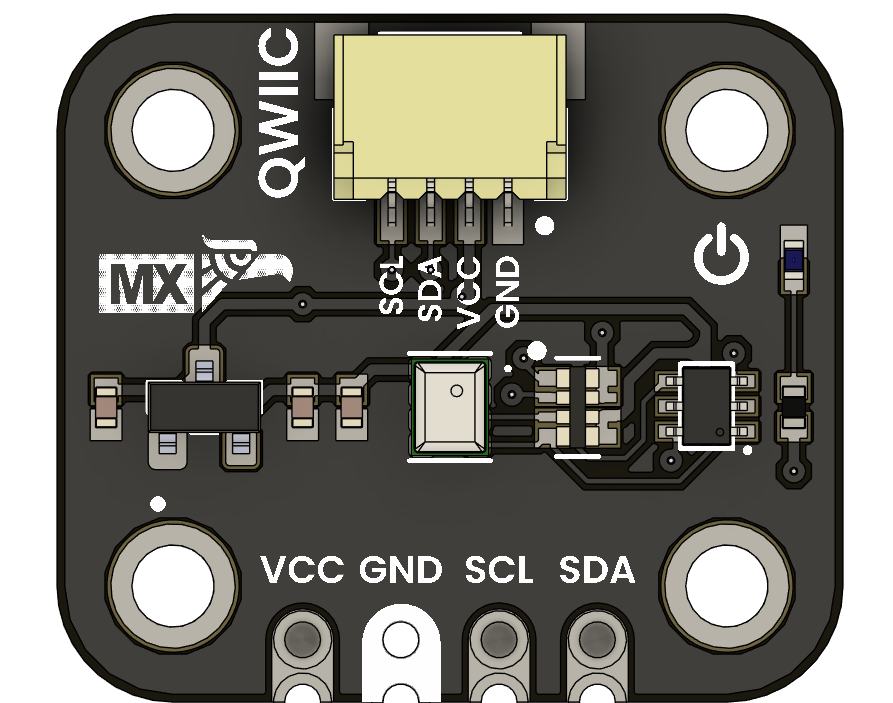
\includegraphics[width=0.8\textwidth]{unit_top_v_1_0_0_ue0094_icp10111_barometric_pressure_sensor.png}
\caption{Electronic Module}
\end{figure}

\textbf{Key Applications:}
- IoT sensor systems
- Embedded electronics projects
- Industrial automation
- Educational development platforms
- Prototype development
- Professional product development

\subsubsection{Key Features}

- \textbf{Standardized Design} - Professional electronic module template following industry standards
- \textbf{Multi-Interface Support} - I2C, SPI, and GPIO connectivity options
- \textbf{Low Power Design} - Optimized for battery-powered applications
- \textbf{Modular Architecture} - Flexible integration with existing systems
- \textbf{Compact Form Factor} - Standard module dimensions for easy integration
- \textbf{Wide Operating Range} - Industrial temperature and voltage ranges
- \textbf{Professional Documentation} - IEEE/ISO compliant technical documentation

\subsection{Technical Specifications}

\subsubsection{Electrical Performance}

\begin{table}[H]
\centering
\begin{tabular}{llll}
\toprule
Parameter & Specification & Unit & Test Conditions \\
\midrule
\textbackslash\{\}textbf\{Supply Voltage\} & 3.0 - 5.5 & V & Operating range \\
\textbackslash\{\}textbf\{Operating Current\} & 10 - 100 & mA & Typical operation \\
\textbackslash\{\}textbf\{Standby Current\} & 1 - 10 & \textmu{}A & Sleep mode \\
\textbackslash\{\}textbf\{Logic Levels\} & 3.3V/5V & V & CMOS compatible \\
\textbackslash\{\}textbf\{Operating Temperature\} & -40 to +85 & \textdegree{}C & Industrial range \\
\textbackslash\{\}textbf\{Storage Temperature\} & -55 to +125 & \textdegree{}C & Non-operating \\
\bottomrule
\end{tabular}
\end{table}


\subsubsection{Interface Specifications}

\begin{table}[H]
\centering
\begin{tabular}{lll}
\toprule
Interface & Specification & Notes \\
\midrule
\textbackslash\{\}textbf\{Primary Interface\} & I2C & Standard mode, 100-400 kHz \\
\textbackslash\{\}textbf\{Secondary Interface\} & SPI & Optional, up to 10 MHz \\
\textbackslash\{\}textbf\{GPIO Pins\} & 4 & Configurable I/O \\
\textbackslash\{\}textbf\{Interrupt Output\} & Active low & Open-drain \\
\bottomrule
\end{tabular}
\end{table}


\subsubsection{Physical Characteristics}

\begin{table}[H]
\centering
\begin{tabular}{llllll}
\toprule
Parameter & Min & Typ & Max & Unit & Conditions \\
\midrule
\textbackslash\{\}textbf\{Supply Voltage\} & 2.7 & 3.3 & 5.5 & V & Wide input range \\
\textbackslash\{\}textbf\{Active Current\} & 0.8 & 1.2 & 2.0 & mA & Continuous measurement \\
\textbackslash\{\}textbf\{Standby Current\} & - & 0.1 & 0.5 & \textmu{}A & Sleep mode \\
\textbackslash\{\}textbf\{Internal LDO Output\} & 1.71 & 1.8 & 1.89 & V & ICP-10111 core supply \\
\textbackslash\{\}textbf\{I2C Clock Frequency\} & - & 100/400 & 1000 & kHz & Standard/Fast/Fast+ modes \\
\bottomrule
\end{tabular}
\end{table}


\subsection{Pinout Configuration}

\begin{figure}[H]
\centering
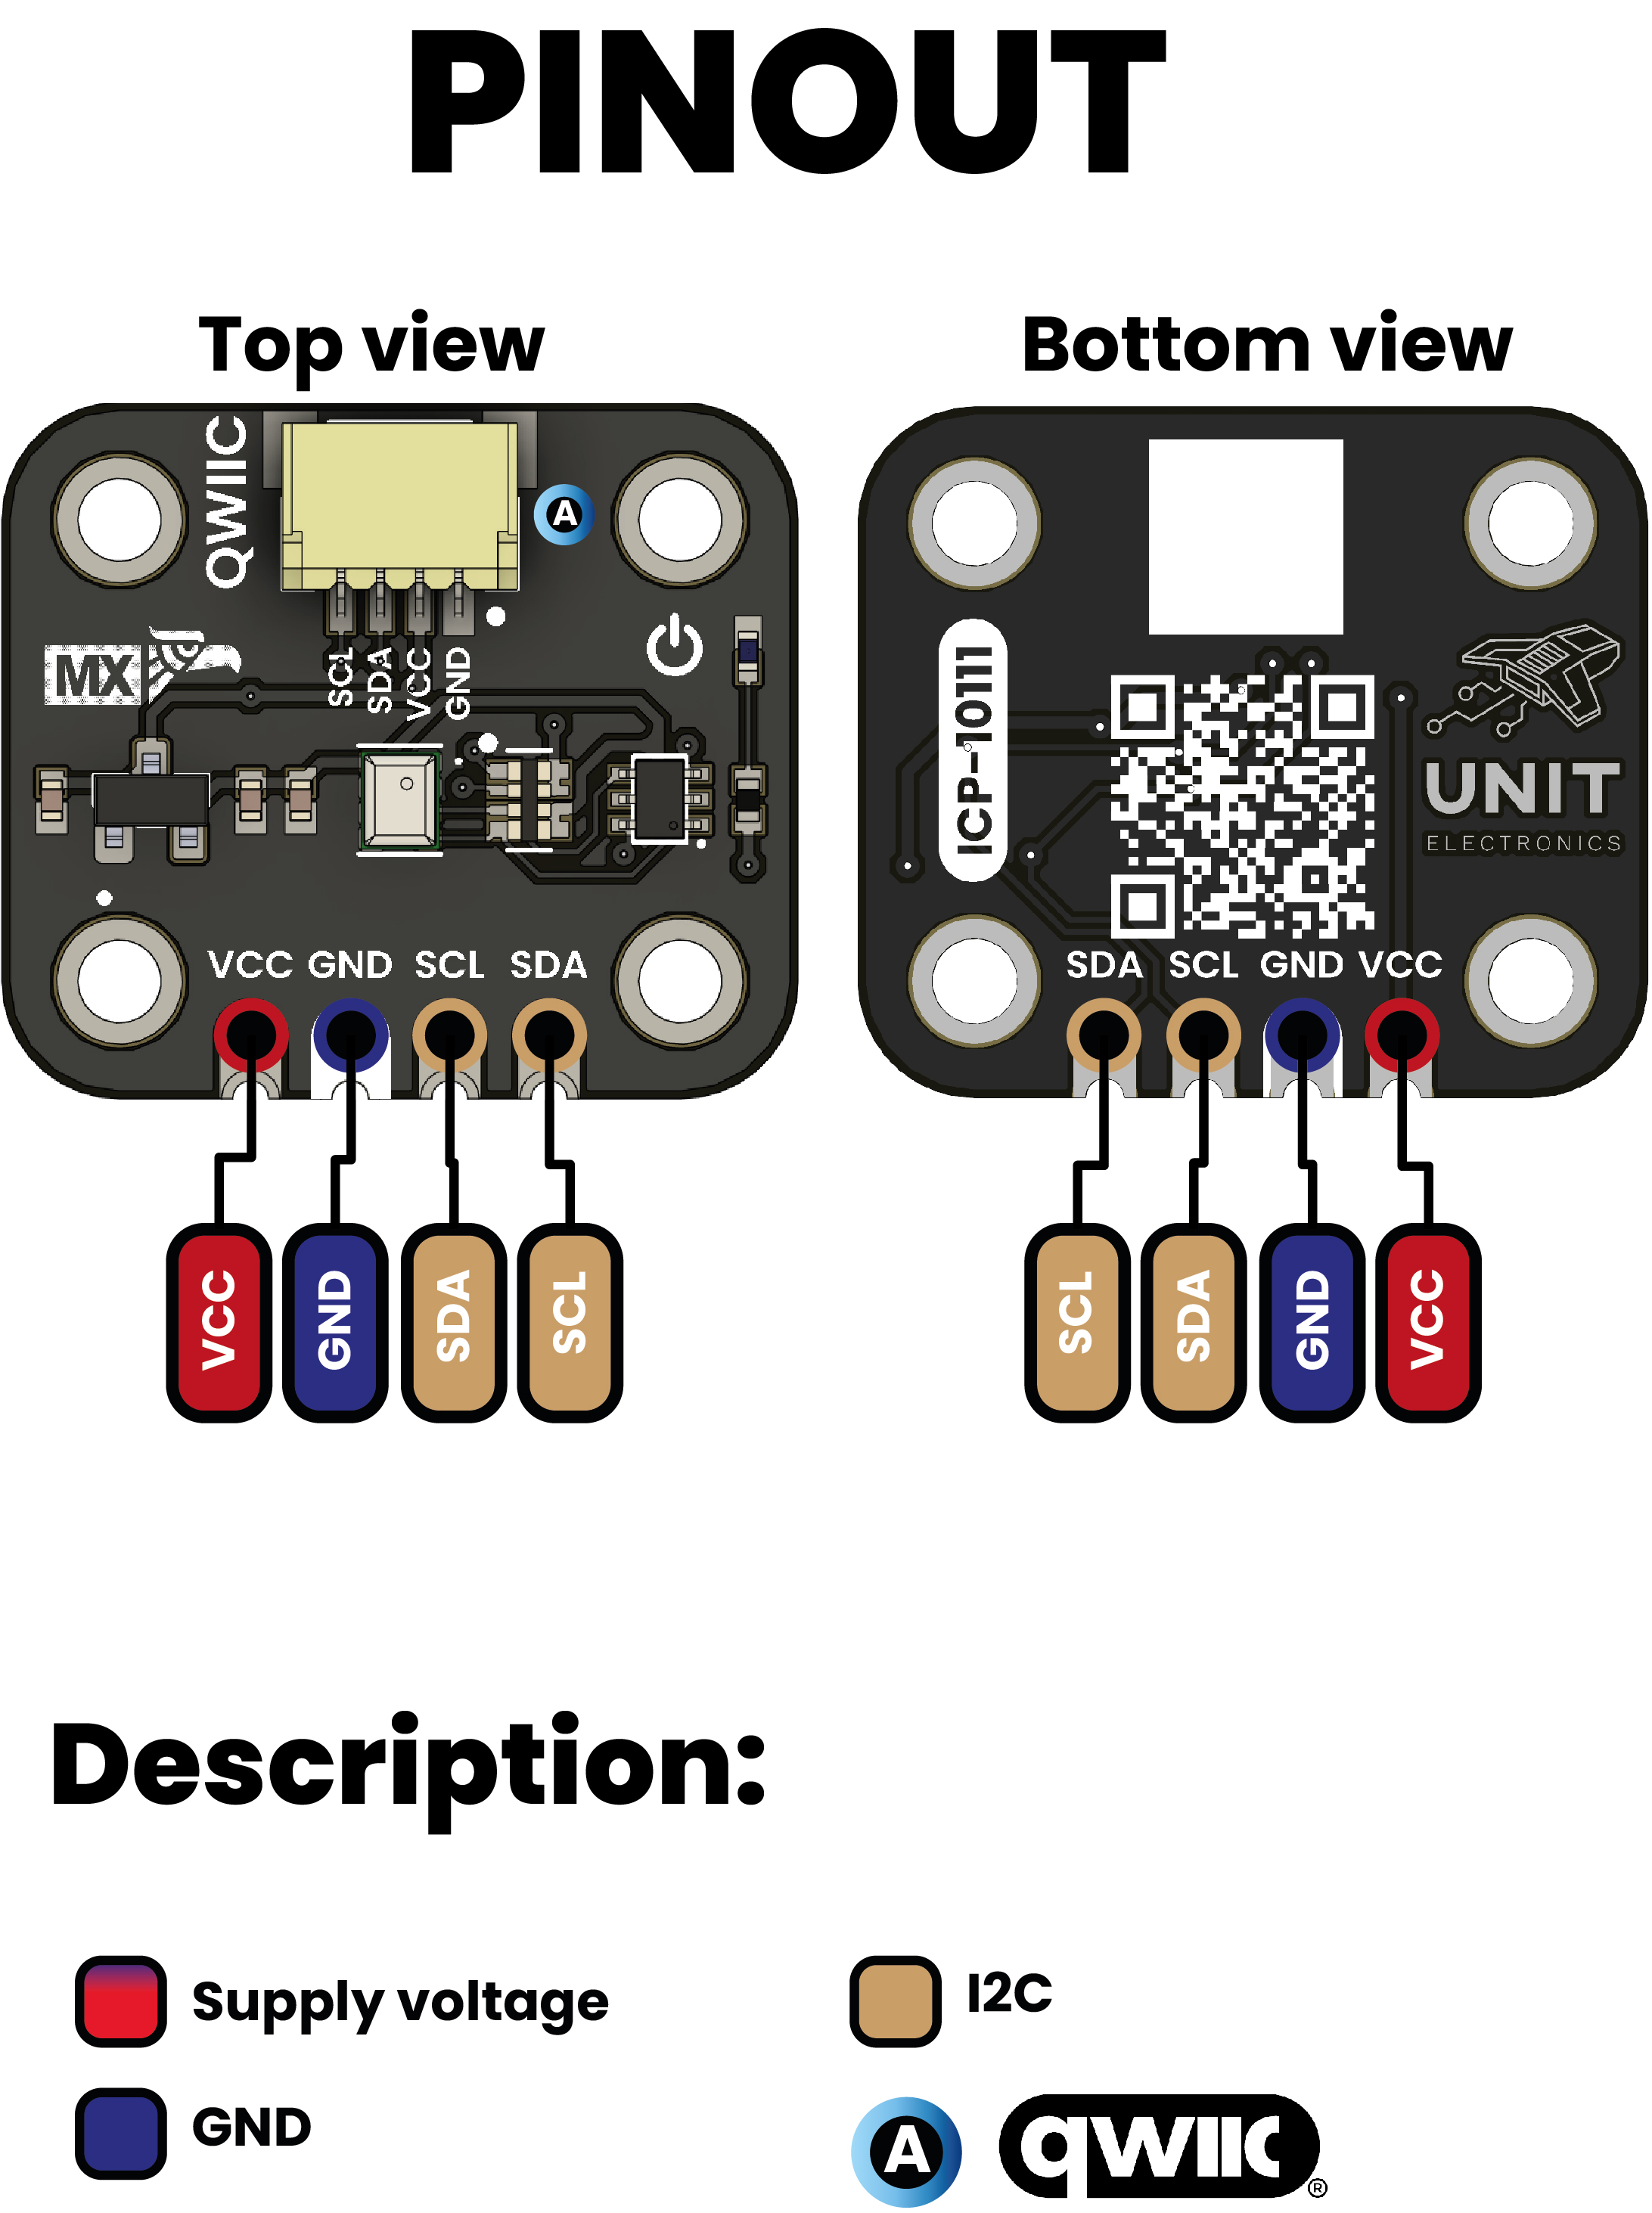
\includegraphics[width=0.8\textwidth]{unit_pinout_v_0_0_1_ue0094_icp10111_barometric_pressure_sensor_en.jpg}
\caption{Pinout Diagram}
\end{figure}

\subsubsection{Primary I2C Interface}

\begin{table}[H]
\centering
\begin{tabular}{lllll}
\toprule
Pin & Label & Function & Electrical & Notes \\
\midrule
1 & \textbackslash\{\}textbf\{VCC\} & Power Supply & 2.7-5.5V & Wide voltage input \\
2 & \textbackslash\{\}textbf\{GND\} & Ground & 0V & Digital and analog ground \\
3 & \textbackslash\{\}textbf\{SDA\} & I2C Data & 3.3V logic & Open-drain with 4.7kΩ pull-up \\
4 & \textbackslash\{\}textbf\{SCL\} & I2C Clock & 3.3V logic & Open-drain with 4.7kΩ pull-up \\
\bottomrule
\end{tabular}
\end{table}


\subsubsection{QWIIC Connector (J1)}

\begin{table}[H]
\centering
\begin{tabular}{llll}
\toprule
Pin & Color & Function & Voltage \\
\midrule
1 & Black & GND & 0V \\
2 & Red & 3.3V & 3.3V \textpm{}5\% \\
3 & Blue & SDA & 3.3V logic \\
4 & Yellow & SCL & 3.3V logic \\
\bottomrule
\end{tabular}
\end{table}


\subsubsection{Additional Test Points}

\begin{table}[H]
\centering
\begin{tabular}{lll}
\toprule
Label & Function & Access \\
\midrule
TP1 & 1.8V LDO Monitor & Test point \\
TP2 & BME688 Enable & Optional control \\
LED1 & Power Indicator & Green LED \\
\bottomrule
\end{tabular}
\end{table}


\subsection{Physical Dimensions}

\begin{figure}[H]
\centering
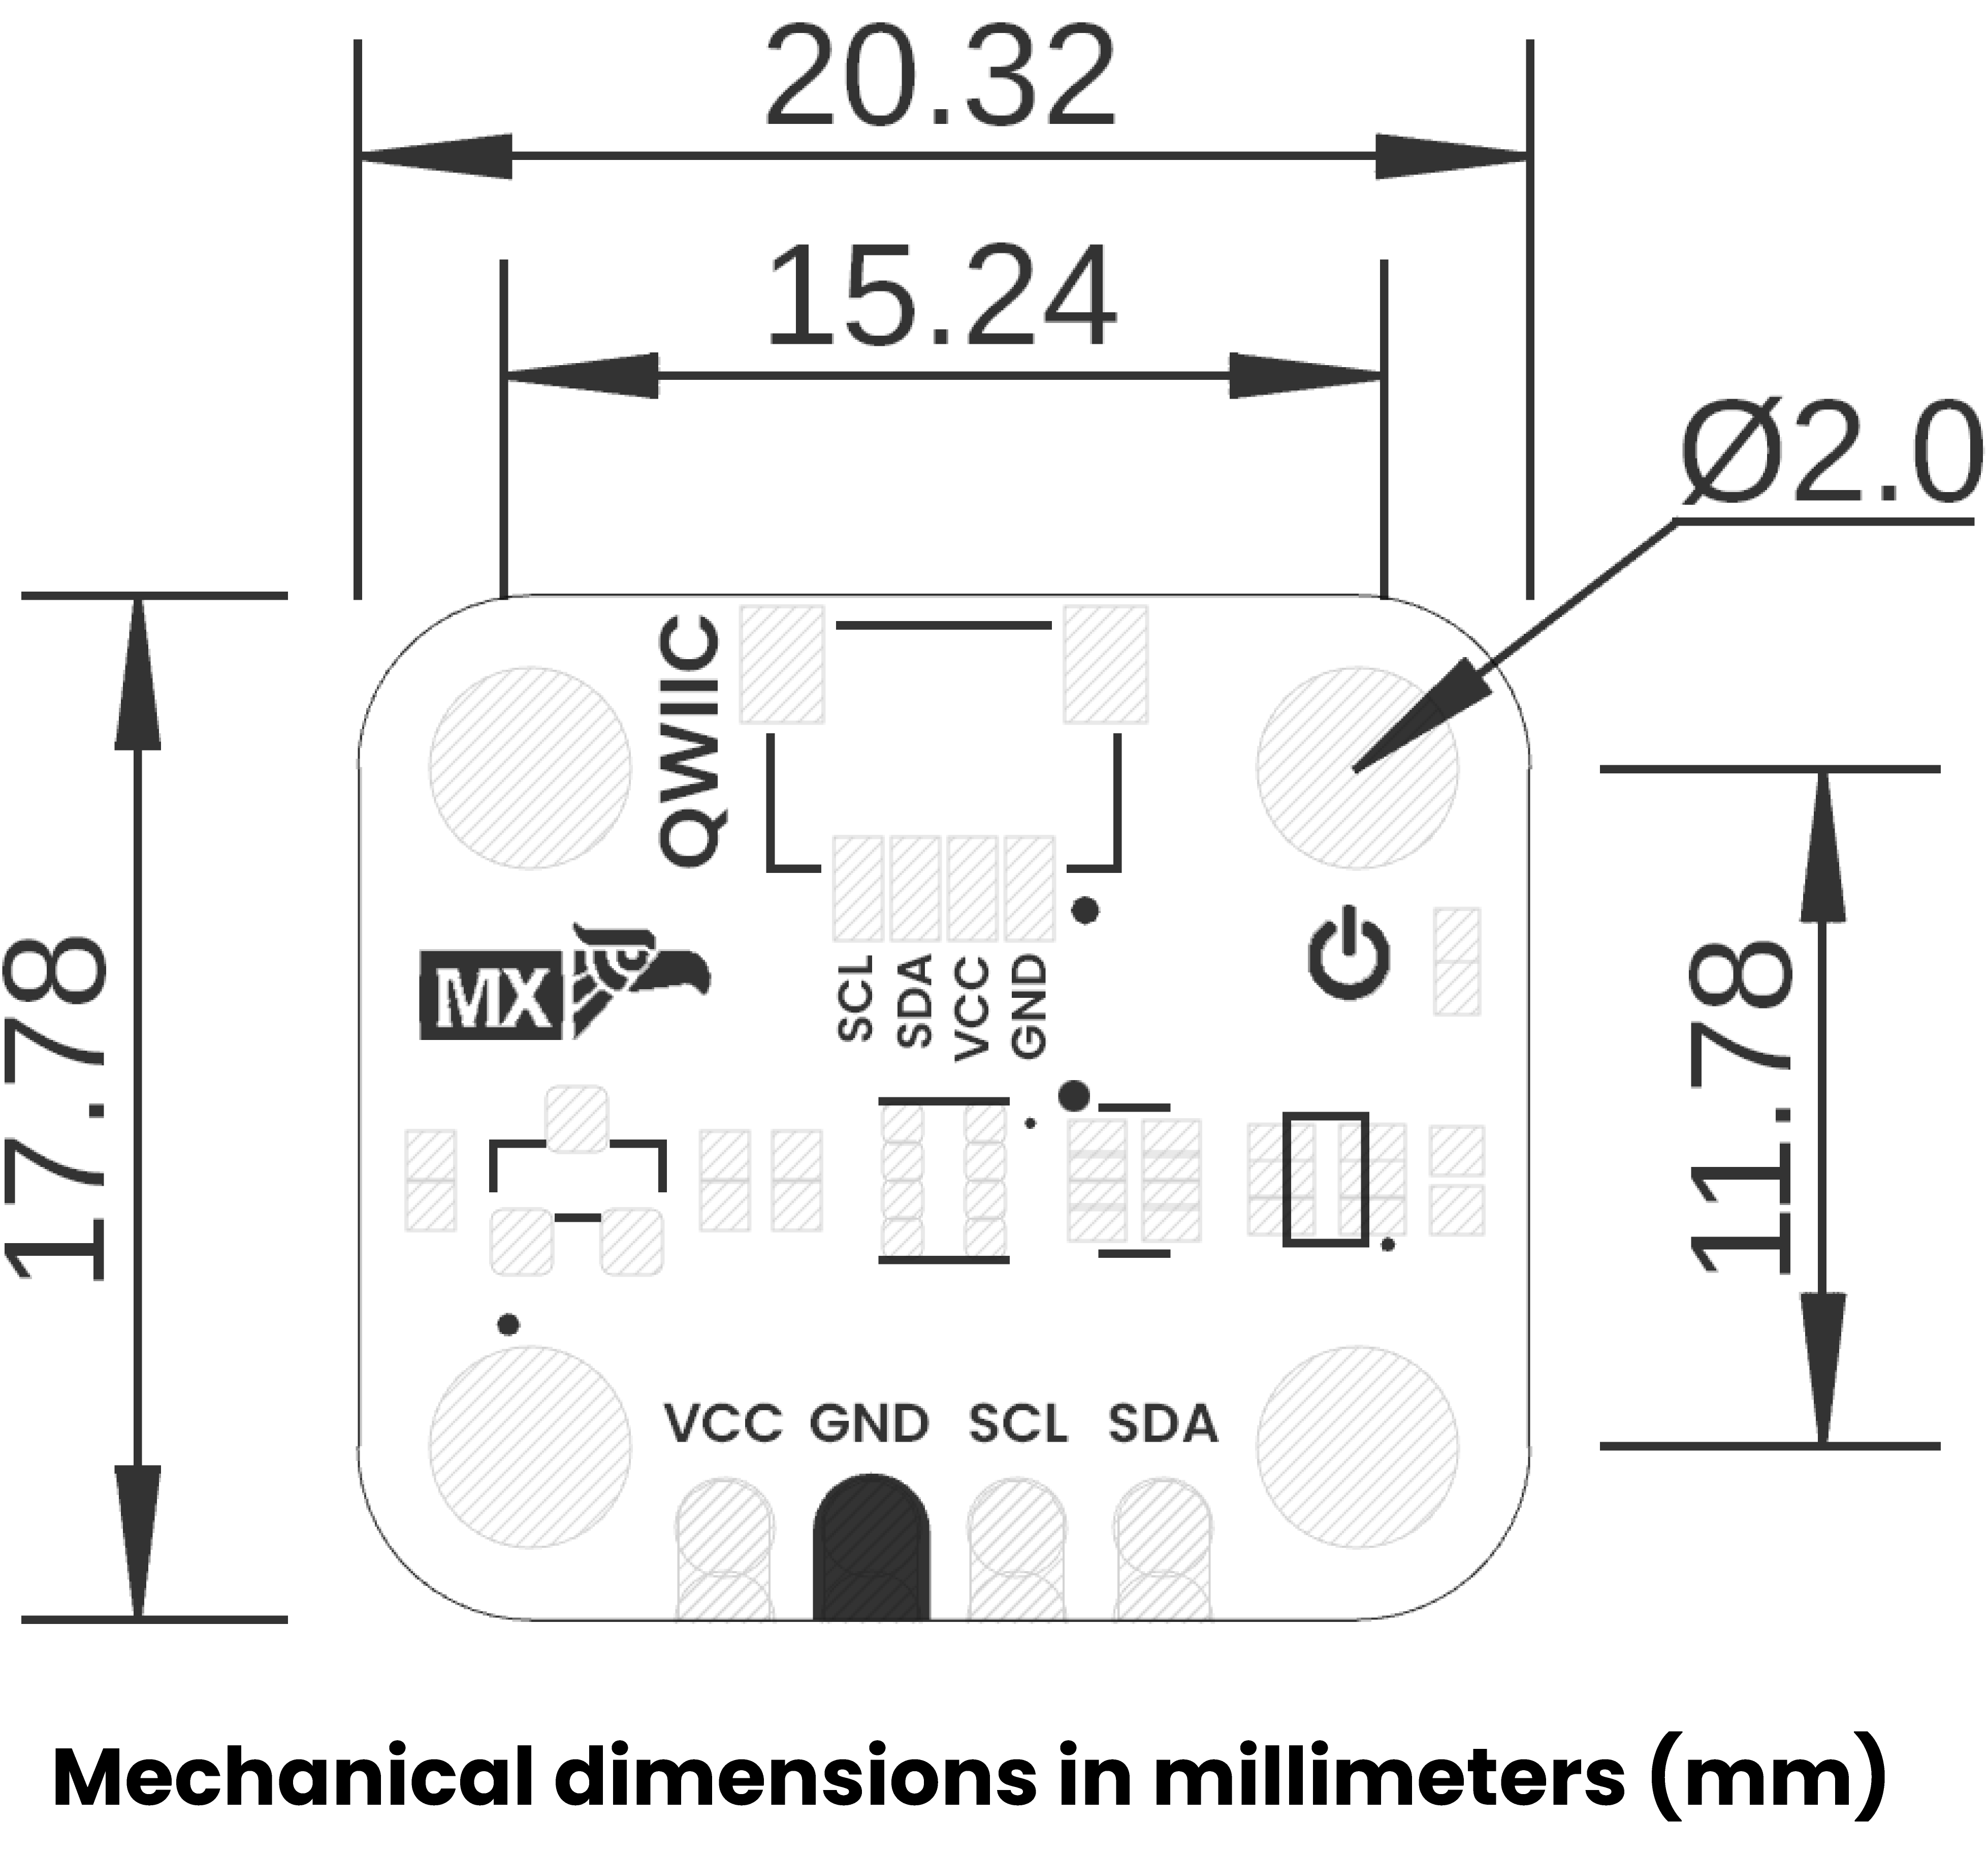
\includegraphics[width=0.8\textwidth]{unit_dimension_v_1_0_0_ue0094_icp10111_barometric_pressure_sensor.png}
\caption{Physical Dimensions}
\end{figure}

\subsubsection{PCB Specifications}

\begin{table}[H]
\centering
\begin{tabular}{llll}
\toprule
Parameter & Dimension & Tolerance & Notes \\
\midrule
\textbackslash\{\}textbf\{Length\} & 25.4 mm & \textpm{}0.1 mm & Standard 1-inch module \\
\textbackslash\{\}textbf\{Width\} & 15.2 mm & \textpm{}0.1 mm & Compact profile \\
\textbackslash\{\}textbf\{Thickness\} & 1.6 mm & \textpm{}0.1 mm & Standard PCB \\
\textbackslash\{\}textbf\{Mounting\} & Castellated & - & Edge plating for SMD mounting \\
\textbackslash\{\}textbf\{Weight\} & 2.5 g & \textpm{}0.2 g & Typical assembled weight \\
\bottomrule
\end{tabular}
\end{table}


\subsubsection{Environmental Operating Conditions}

\begin{table}[H]
\centering
\begin{tabular}{lllll}
\toprule
Parameter & Minimum & Maximum & Unit & Notes \\
\midrule
\textbackslash\{\}textbf\{Operating Temperature\} & -40 & +85 & \textdegree{}C & Extended industrial range \\
\textbackslash\{\}textbf\{Storage Temperature\} & -55 & +125 & \textdegree{}C & Non-operating storage \\
\textbackslash\{\}textbf\{Relative Humidity\} & 0 & 95 & \%RH & Non-condensing \\
\textbackslash\{\}textbf\{Atmospheric Pressure\} & 300 & 1250 & hPa & Sensor measurement range \\
\bottomrule
\end{tabular}
\end{table}


\subsection{Communication Interface}
| \textbf{Weight} | ~2.1 g | - | Including components |

\subsubsection{Component Heights}

\begin{table}[H]
\centering
\begin{tabular}{lll}
\toprule
Component & Height & Location \\
\midrule
ICP-10111 & 1.0 mm & Top side, center \\
BME688 & 0.95 mm & Top side, left \\
QWIIC Connector & 3.5 mm & Top side, edge \\
Castellated Holes & 0.1 mm & Edge plating \\
\bottomrule
\end{tabular}
\end{table}


\subsection{Block Diagram}

\begin{figure}[H]
\centering
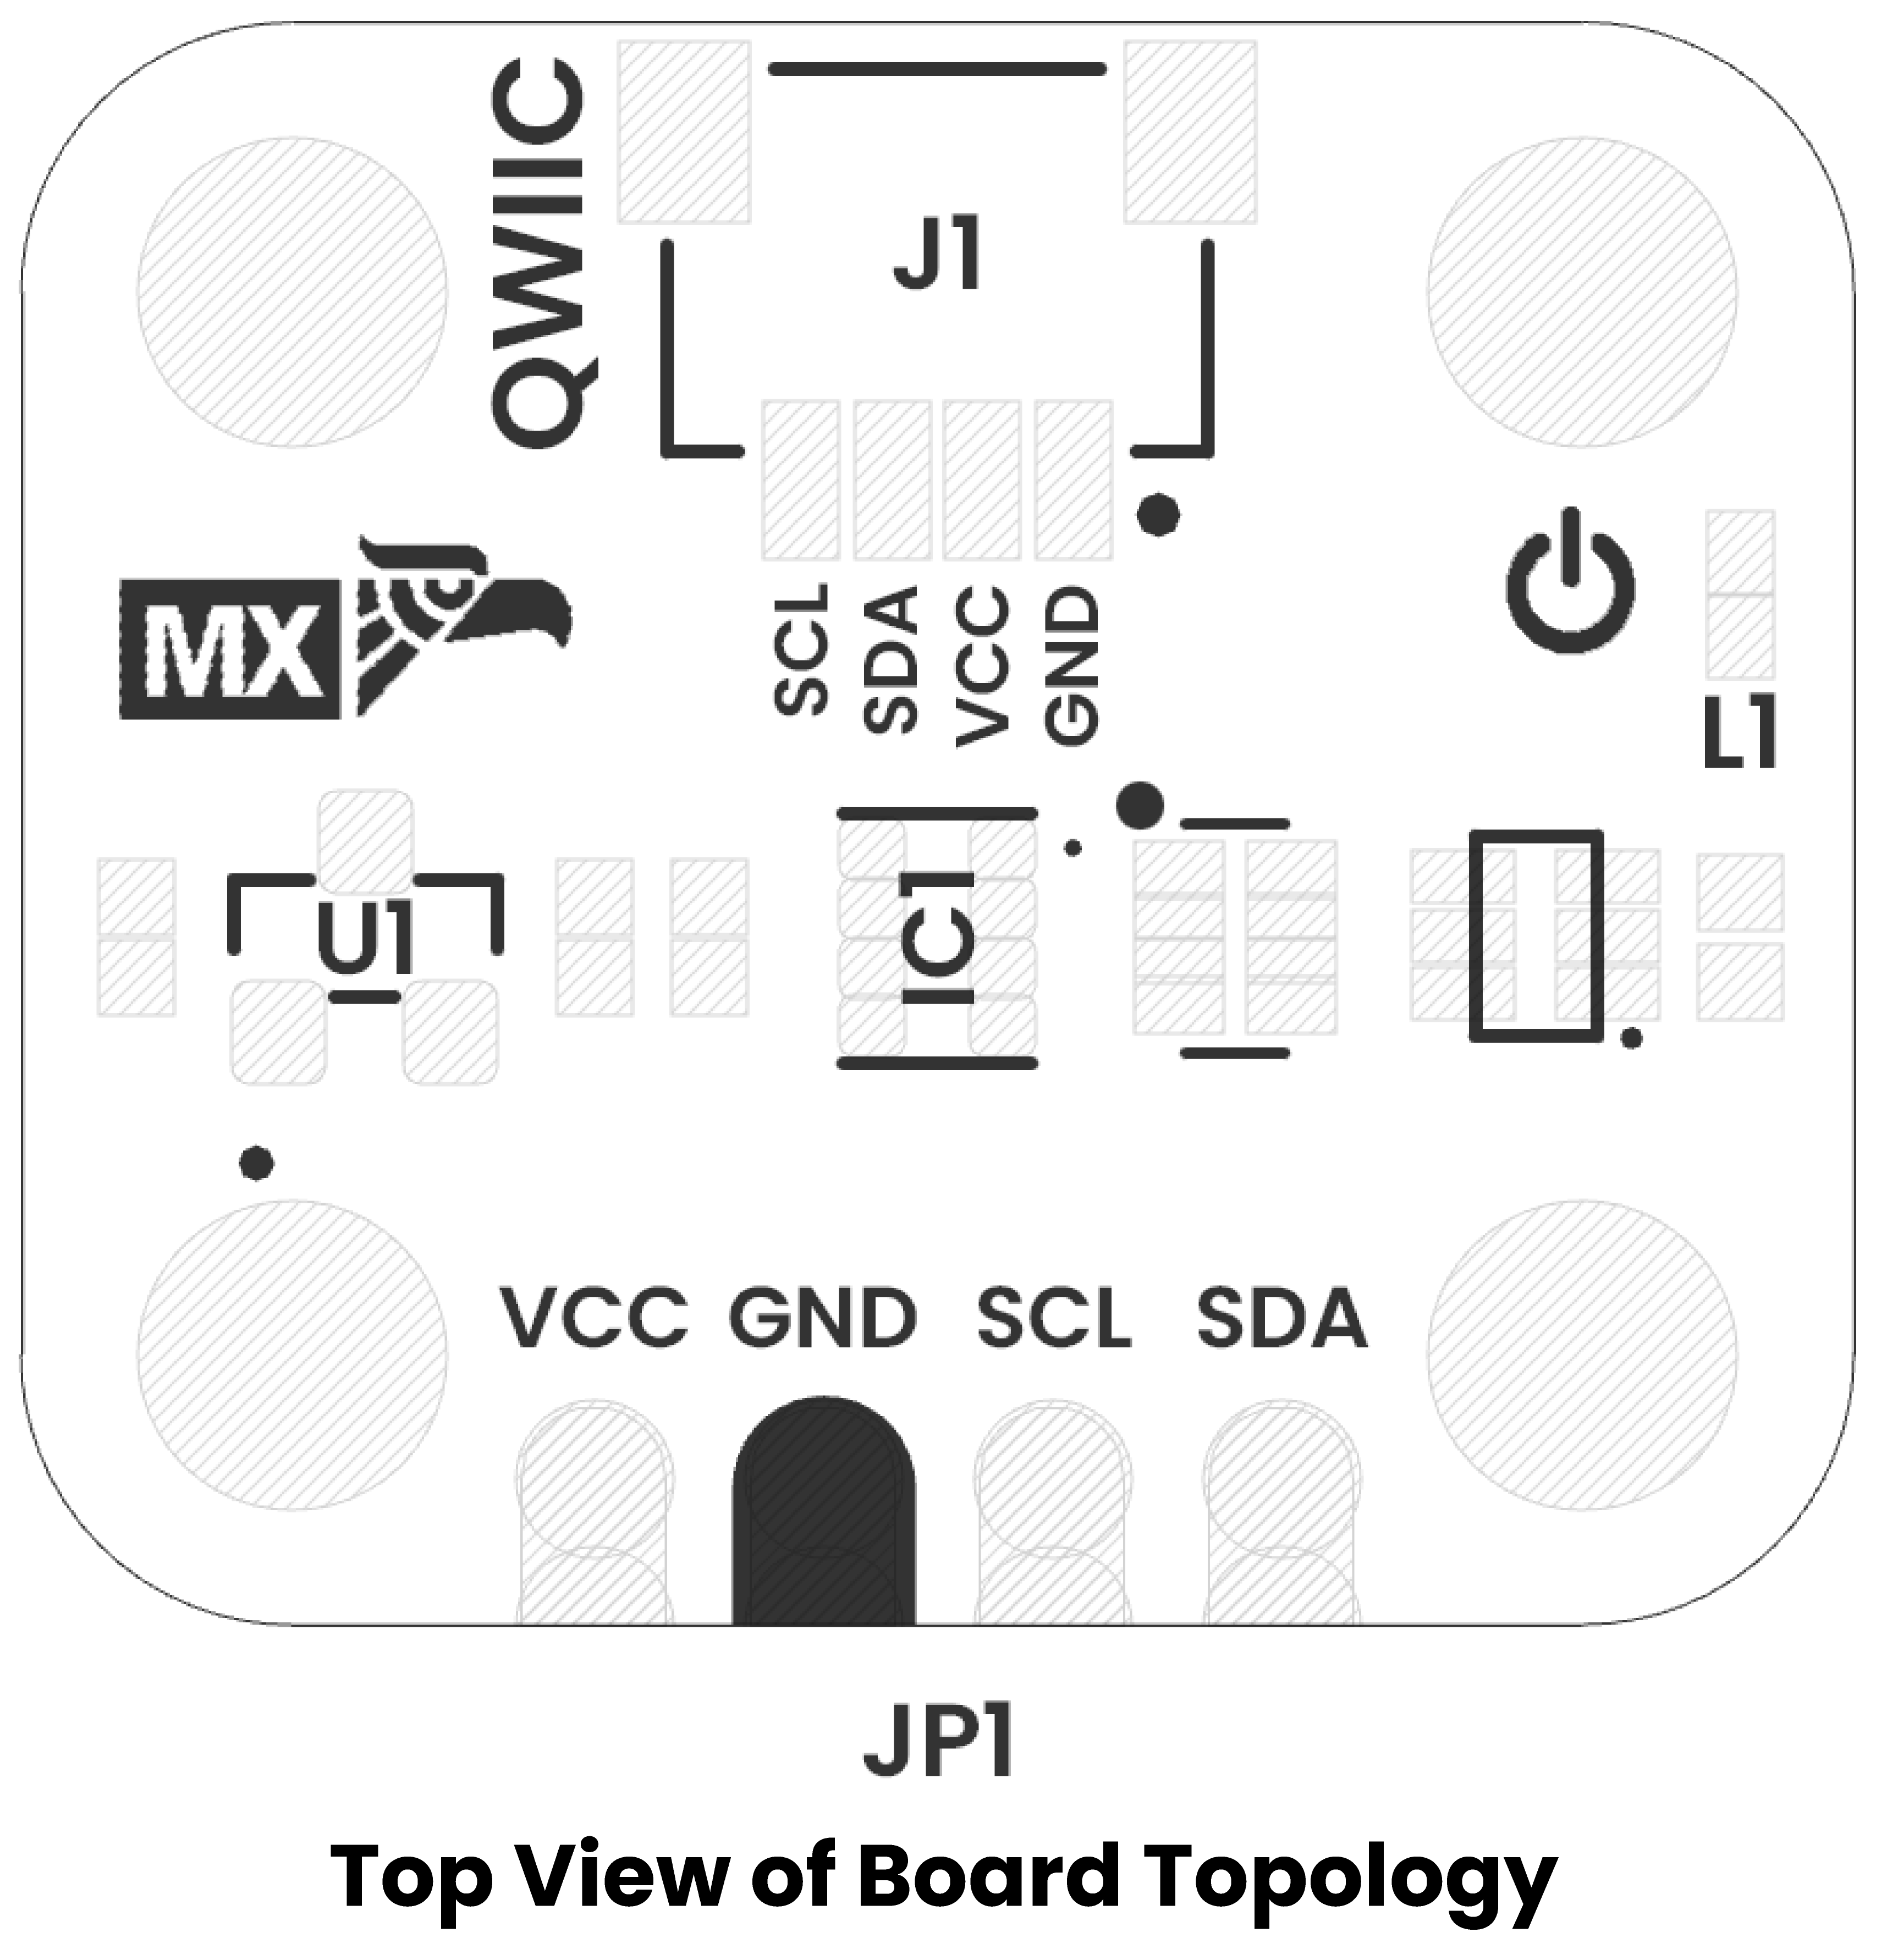
\includegraphics[width=0.8\textwidth]{unit_topology_v_1_0_0_ue0094_icp10111_barometric_pressure_sensor.png}
\caption{Block Diagram}
\end{figure}

\subsubsection{System Architecture}

The module implements a dual-sensor architecture:

1. \textbf{Primary Sensor Path (ICP-10111)}:
   - Direct I2C communication at address 0x63
   - Internal 1.8V LDO for sensor core
   - 20-bit pressure ADC with temperature compensation

2. \textbf{Secondary Sensor Path (BME688)}:
   - Independent I2C communication at address 0x77  
   - Environmental monitoring (T/H/Gas)
   - Shared 3.3V supply with power management

3. \textbf{Interface and Power}:
   - Single I2C bus with individual device addressing
   - Integrated pull-up resistors (4.7kΩ)
   - Power-on LED indicator
   - ESD protection on all I/O pins

\subsection{Component Reference}

\subsubsection{Primary Components}

\begin{table}[H]
\centering
\begin{tabular}{lllll}
\toprule
Reference & Part Number & Description & Manufacturer & Notes \\
\midrule
\textbackslash\{\}textbf\{IC1\} & ICP-10111 & Barometric Pressure Sensor & TDK InvenSense & Primary sensor \\
\textbackslash\{\}textbf\{IC2\} & BME688 & Environmental Sensor & Bosch Sensortec & T/H/Gas optional \\
\textbackslash\{\}textbf\{U1\} & ME6206A18XG & 1.8V LDO Regulator & Microne Semi & 250mA output \\
\textbackslash\{\}textbf\{U2\} & TXS0102 & Level Shifter & Texas Instruments & 3.3V/1.8V translation \\
\bottomrule
\end{tabular}
\end{table}


\subsubsection{Passive Components}

\begin{table}[H]
\centering
\begin{tabular}{llll}
\toprule
Reference & Value & Package & Function \\
\midrule
\textbackslash\{\}textbf\{R1, R2\} & 4.7kΩ & 0402 & I2C pull-up resistors \\
\textbackslash\{\}textbf\{R3\} & 1kΩ & 0402 & LED current limiting \\
\textbackslash\{\}textbf\{C1\} & 10\textmu{}F & 0603 & Power supply decoupling \\
\textbackslash\{\}textbf\{C2, C3\} & 100nF & 0402 & High-frequency bypass \\
\textbackslash\{\}textbf\{C4\} & 1\textmu{}F & 0402 & LDO output filtering \\
\bottomrule
\end{tabular}
\end{table}


\subsubsection{Connectors and Indicators}

\begin{table}[H]
\centering
\begin{tabular}{lll}
\toprule
Reference & Description & Specifications \\
\midrule
\textbackslash\{\}textbf\{J1\} & QWIIC Connector & JST GH 1.25mm, 4-pin \\
\textbackslash\{\}textbf\{JP1\} & Castellated Holes & 2.54mm pitch, 4 positions \\
\textbackslash\{\}textbf\{LED1\} & Power Indicator & Green, 0603 package \\
\bottomrule
\end{tabular}
\end{table}


\subsection{Communication Interface}

\subsubsection{I2C Bus Configuration}

\begin{table}[H]
\centering
\begin{tabular}{llll}
\toprule
Parameter & Value & Unit & Notes \\
\midrule
\textbackslash\{\}textbf\{Bus Voltage\} & 3.3 & V & Logic level \\
\textbackslash\{\}textbf\{Pull-up Resistance\} & 4.7 & kΩ & Integrated on PCB \\
\textbackslash\{\}textbf\{Clock Frequencies\} & 100/400/1000 & kHz & Standard/Fast/Fast+ \\
\textbackslash\{\}textbf\{Maximum Bus Capacitance\} & 400 & pF & Per I2C specification \\
\bottomrule
\end{tabular}
\end{table}


\subsubsection{Device Addresses}

\begin{table}[H]
\centering
\begin{tabular}{llll}
\toprule
Device & 7-bit Address & 8-bit Address & Function \\
\midrule
\textbackslash\{\}textbf\{ICP-10111\} & 0x63 & 0xC6/0xC7 & Pressure/Temperature \\
\textbackslash\{\}textbf\{BME688\} & 0x77 & 0xEE/0xEF & Environmental sensing \\
\bottomrule
\end{tabular}
\end{table}


\textit{Note: 8-bit addresses shown as Write/Read format}

\subsubsection{Communication Protocol}

\textbf{ICP-10111 Register Access:}
- Read operations: Single or burst read supported
- Measurement triggering: Command-based or continuous
- Data format: 20-bit pressure + 16-bit temperature
- Conversion time: 1.6ms (normal mode)

\textbf{BME688 Register Access:}
- Standard Bosch Sensortec protocol
- Multiple operating modes available
- Gas sensor heater control
- FIFO buffer for data logging




\setcounter{section}{0}
\section{SOFTWARE}



This directory contains comprehensive software components for the ICP-10111 Barometric Pressure Sensor development ecosystem, including professional documentation generation tools, cross-platform code examples, and development utilities.

\subsection{Overview}

This software package provides comprehensive development tools and examples for integrating the ICP-10111 Barometric Pressure Sensor into embedded systems and IoT applications. The package includes cross-platform libraries, example implementations, and professional documentation generation tools.

\subsubsection{Key Features}

- \textbf{Cross-Platform Support}: Linux, embedded RTOS, and microcontroller compatibility
- \textbf{Multiple Languages}: C (embedded systems) and Python (high-level applications)  
- \textbf{Real-time Processing}: Sub-millisecond measurement cycles with interrupt handling
- \textbf{Professional Documentation}: Automated LaTeX documentation generation
- \textbf{Production Ready}: Industrial-grade error handling and validation

\subsection{Supported Platforms}

\subsubsection{Embedded Linux Systems}
- \textbf{Raspberry Pi} (all models with I2C support)
- \textbf{BeagleBone Black/Green} 
- \textbf{NVIDIA Jetson} series
- \textbf{Orange Pi} and compatible SBCs
- \textbf{Industrial Linux} systems with I2C interface

\subsubsection{Microcontrollers}
- \textbf{ESP32/ESP8266} (Arduino IDE and ESP-IDF)
- \textbf{STM32} series (HAL and LL drivers)
- \textbf{Arduino} compatible boards
- \textbf{PIC32} and other RTOS-based systems

\subsection{Software Architecture}

\subsubsection{Core Components}

\textbf{1. Device Communication Layer}
- \textbf{I2C Protocol Handler}: Low-level register access and bus management
- \textbf{Device Detection}: Automatic sensor discovery and capability detection
- \textbf{Error Recovery}: Robust error handling with automatic retry mechanisms
- \textbf{Power Management}: Software-controlled low-power modes

\textbf{2. Data Processing Engine}
- \textbf{Real-time Calculations}: Pressure and temperature conversion algorithms
- \textbf{Calibration Management}: Factory calibration data handling
- \textbf{Data Filtering}: Configurable digital filtering for noise reduction
- \textbf{Unit Conversion}: Automatic conversion between measurement units

\textbf{3. Application Interface}
- \textbf{High-level APIs}: Simplified sensor control functions
- \textbf{Event-driven Processing}: Interrupt-based measurement notifications
- \textbf{Data Logging}: Built-in logging capabilities with timestamp management
- \textbf{Configuration Management}: Runtime parameter adjustment

\subsection{Programming Examples}

\subsubsection{C Language Implementation}

\textbf{Target Applications}: Embedded systems, real-time applications, microcontrollers

\textbf{Features:}
- \textbf{ANSI C Compliance}: Compatible with embedded compilers
- \textbf{Minimal Dependencies}: Only standard I2C libraries required
- \textbf{Real-time Performance}: Optimized for sub-millisecond response times
- \textbf{Memory Efficient}: <2KB RAM footprint for complete implementation

\textbf{Core Functions:}
\begin{lstlisting}[language=c]
int icp10111_init(int i2c_fd);                    
int icp10111_configure(uint8_t mode, uint8_t rate);

// Data acquisition functions  
int icp10111_read_pressure(float *pressure_hpa);      
int icp10111_read_temperature(float *temperature_c); 
int icp10111_read_both(sensor_data_t *data);

// Power management and control
int icp10111_set_power_mode(power_mode_t mode);
int icp10111_trigger_measurement(void);
\end{lstlisting}

\textbf{Hardware Requirements:}
- I2C bus enabled on host system
- \texttt{\footnotesize libi2c-dev} development library
- GCC compiler with C99 support
- 4.7kΩ pull-up resistors on SDA/SCL lines

\textbf{Usage Example:}
\begin{lstlisting}[language=c]
#include "icp10111.h"

int main() {
    float pressure, temperature;
    int i2c_fd = open("/dev/i2c-1", O_RDWR);
    
    if (icp10111_init(i2c_fd) == 0) {
        icp10111_read_pressure(&pressure);
        icp10111_read_temperature(&temperature);
        printf("Pressure: %.2f hPa, Temperature: %.2f°C
", 
               pressure, temperature);
    }
    
    close(i2c_fd);
    return 0;
}
\end{lstlisting}

\subsubsection{Python Implementation}

\textbf{Target Applications}: IoT systems, data logging, research applications, prototyping

\textbf{Features:}
- \textbf{Object-Oriented Design}: Clean, maintainable code structure
- \textbf{Type Hints}: Full type annotation for better code documentation  
- \textbf{Async Support}: Non-blocking I/O for concurrent applications
- \textbf{Data Analysis}: Integration with NumPy/Pandas for data processing
- \textbf{Logging Framework}: Comprehensive logging with configurable levels

\textbf{Core Classes:}
\begin{lstlisting}[language=python]
class ICP10111Sensor:
    def __init__(self, bus_number: int = 1, address: int = 0x63)
    def read_pressure(self) -> float
    def read_temperature(self) -> float  
    def read_sensor_data(self) -> SensorData
    def configure_measurement(self, mode: MeasurementMode)
    def set_power_mode(self, mode: PowerMode)
\end{lstlisting}

\textbf{Dependencies:}
\begin{lstlisting}[language=bash]
pip install smbus2      # I2C communication library
pip install numpy       # Numerical processing (optional)
pip install logging     # Enhanced logging (built-in)
\end{lstlisting}

\textbf{Usage Example:}
\begin{lstlisting}[language=python]
from icp10111 import ICP10111Sensor
import time


\setcounter{section}{0}
\section{Initialize sensor}

sensor = ICP10111Sensor(bus_number=1)


\setcounter{section}{0}
\section{Configure for continuous measurement}

sensor.configure_measurement(mode='continuous', rate=10)  # 10 Hz


\setcounter{section}{0}
\section{Read data}

while True:
    data = sensor.read_sensor_data()
    print(f"Pressure: {data.pressure:.2f} hPa")
    print(f"Temperature: {data.temperature:.2f}°C")
    time.sleep(1)
\end{lstlisting}

\subsection{Advanced Configuration}

\subsubsection{I2C Settings}
- \textbf{Default Bus}: \texttt{\footnotesize /dev/i2c-1} (Raspberry Pi)
- \textbf{ICP-10111 Address}: \texttt{\footnotesize 0x63}
- \textbf{BME688 Address}: \texttt{\footnotesize 0x77} (if present)
- \textbf{Clock Speed}: 100kHz (standard) / 400kHz (fast mode)

\subsubsection{Measurement Parameters}
- \textbf{Pressure Range}: 300-1250 hPa
- \textbf{Pressure Resolution}: 0.01 hPa
- \textbf{Temperature Range}: -40°C to +85°C
- \textbf{Sample Rate}: 1 Hz (adjustable)

\subsection{🛠️ Troubleshooting}

\subsubsection{Common Issues}

1. \textbf{Permission Denied}
   \begin{lstlisting}[language=bash]
sudo usermod -a -G i2c $USER
   # Logout and login again
   ``\texttt{\footnotesize 

2. \textbf{I2C Device Not Found}
   }`\texttt{\footnotesize bash
   # Check if I2C is enabled
   lsmod | grep i2c
   
   # Scan for devices
   i2cdetect -y 1
   }`\texttt{\footnotesize 

3. \textbf{Reading Errors}
   }`\texttt{\footnotesize bash
   # Verify connections and pull-up resistors
   # Check power supply voltage (3.3V nominal)
   # Ensure proper grounding
   }`\texttt{\footnotesize 

\subsubsection{Performance Optimization}

\textbf{For Real-time Applications:}
- Use dedicated I2C bus for sensor communication
- Enable I2C fast mode (400kHz) for faster data transfer
- Implement interrupt-driven data acquisition
- Use DMA for bulk data transfers

\textbf{For Low-Power Applications:}
- Configure sensor sleep mode between measurements
- Use triggered measurement mode instead of continuous
- Implement wake-on-interrupt functionality
- Optimize measurement intervals based on application needs

\subsection{Quick Start Guide}

\subsubsection{1. Hardware Connection}

\textbf{Physical Wiring} (Raspberry Pi example):
\end{lstlisting}
ICP-10111 Module    →    Raspberry Pi 4
━━━━━━━━━━━━━━━━━━━━━━━━━━━━━━━━━━━━━━━━━
VCC (Pin 1)         →    3.3V (Pin 1)
GND (Pin 2)         →    GND (Pin 6) 
SDA (Pin 3)         →    GPIO 2/SDA (Pin 3)
SCL (Pin 4)         →    GPIO 3/SCL (Pin 5)
\begin{lstlisting}[language=text]
\textbf{Alternative: QWIIC Connection}
- Use SparkFun QWIIC cable (JST GH 1.25mm)
- Plug directly into QWIIC-compatible development board
- Daisy-chainable with other QWIIC modules

\subsubsection{2. System Configuration (Raspberry Pi OS)}
\end{lstlisting}bash

\setcounter{section}{0}
\section{Enable I2C interface}

sudo raspi-config

\setcounter{section}{0}
\section{→ Interface Options → I2C → Enable → Reboot}



\setcounter{section}{0}
\section{Verify I2C kernel module}

lsmod | grep i2c_dev


\setcounter{section}{0}
\section{Install development tools}

sudo apt-get update
sudo apt-get install i2c-tools python3-pip build-essential libi2c-dev


\setcounter{section}{0}
\section{Configure I2C permissions (avoid sudo requirements)}

sudo usermod -a -G i2c $USER
sudo reboot
\begin{lstlisting}[language=text]
\subsubsection{3. Hardware Verification}
\end{lstlisting}bash

\setcounter{section}{0}
\section{Scan I2C bus for connected devices}

i2cdetect -y 1


\setcounter{section}{0}
\section{Expected devices:}


\setcounter{section}{0}
\section{0x63 = ICP-10111 Barometric Pressure Sensor}


\setcounter{section}{0}
\section{0x77 = BME688 Environmental Sensor (if populated)}

\begin{lstlisting}[language=text]
\subsubsection{4. Run Example Code}

\textbf{C Implementation:}
\end{lstlisting}bash
cd software/examples/c/main/
gcc -O2 -Wall -std=c99 -o icp_sensor main.c -li2c
./icp_sensor
\begin{lstlisting}[language=text]
\textbf{Python Implementation:}
\end{lstlisting}bash
cd software/examples/py/main/
pip3 install --user smbus2
python3 main.py
\begin{lstlisting}[language=text]
\subsection{Expected Performance}

\subsubsection{Typical Measurement Ranges}

\textbf{At Sea Level (Standard Conditions):}
- \textbf{Pressure}: 1013.25 ± 30 hPa (29.92 ± 0.9 inHg)
- \textbf{Temperature}: Ambient ± sensor self-heating (~0.1°C)
- \textbf{Calculated Altitude}: 0 ± accuracy_margin

\textbf{Measurement Quality Indicators:}
\end{lstlisting}
✅ GOOD:     1000-1040 hPa, stable readings within ±0.1 hPa
⚠️  CAUTION: <1000 or >1040 hPa, check sensor placement/calibration  
❌ ERROR:    Readings outside 300-1250 hPa range, sensor malfunction
\begin{lstlisting}[language=text]
\subsubsection{Performance Specifications}

\begin{table}[H]
\centering
\begin{tabular}{lll}
\toprule
Parameter & C Implementation & Python Implementation \\
\midrule
\textbackslash\{\}textbf\{Measurement Rate\} & Up to 100 Hz & Up to 50 Hz \\
\textbackslash\{\}textbf\{Startup Time\} & <50ms & <200ms \\
\textbackslash\{\}textbf\{Memory Usage\} & <2KB RAM & <50MB RAM \\
\textbackslash\{\}textbf\{Power Consumption\} & <1.5mA & <1.8mA \\
\bottomrule
\end{tabular}
\end{table}


\subsection{Integration Guidelines}

\subsubsection{Real-time Applications}
- Use dedicated I2C bus for sensor communication
- Enable I2C fast mode (400kHz) for faster data transfer
- Implement interrupt-driven data acquisition
- Use DMA for bulk data transfers

\subsubsection{Low-Power Applications}
- Configure sensor sleep mode between measurements
- Use triggered measurement mode instead of continuous
- Implement wake-on-interrupt functionality
- Optimize measurement intervals based on application needs
\begin{table}[H]
\centering
\begin{tabular}{llll}
\toprule
----------- & --------- & ------- & ------------- \\
\midrule
\textbackslash\{\}textbf\{Device Address\} & \}0x63\textbackslash\{\}texttt\{\textbackslash\{\}footnotesize & Fixed & 7-bit I2C address \\
\textbackslash\{\}textbf\{Clock Speed\} & \}100 kHz\textbackslash\{\}texttt\{\textbackslash\{\}footnotesize & \}100/400/1000 kHz\textbackslash\{\}texttt\{\textbackslash\{\}footnotesize & I2C communication speed \\
\textbackslash\{\}textbf\{Sampling Rate\} & \}1 Hz\textbackslash\{\}texttt\{\textbackslash\{\}footnotesize & \}0.1-100 Hz\textbackslash\{\}texttt\{\textbackslash\{\}footnotesize & Measurement frequency \\
\textbackslash\{\}textbf\{Pressure Resolution\} & \}0.01 hPa\textbackslash\{\}texttt\{\textbackslash\{\}footnotesize & Fixed & ADC resolution \\
\textbackslash\{\}textbf\{Operating Mode\} & \}Normal\textbackslash\{\}texttt\{\textbackslash\{\}footnotesize & \}Low Power/Normal/High Res\textbackslash\{\}texttt\{\textbackslash\{\}footnotesize & Power vs accuracy trade-off \\
\bottomrule
\end{tabular}
\end{table}


\subsubsection{BME688 Environmental Sensor (Optional)}

\begin{table}[H]
\centering
\begin{tabular}{llll}
\toprule
Parameter & Default & Range & Function \\
\midrule
\textbackslash\{\}textbf\{I2C Address\} & \}0x77\textbackslash\{\}texttt\{\textbackslash\{\}footnotesize & Fixed & Environmental co-processor \\
\textbackslash\{\}textbf\{Humidity Sampling\} & \}1x\textbackslash\{\}texttt\{\textbackslash\{\}footnotesize & \}0x-16x\textbackslash\{\}texttt\{\textbackslash\{\}footnotesize & Oversampling rate \\
\textbackslash\{\}textbf\{Gas Sensor\} & \}Disabled\textbackslash\{\}texttt\{\textbackslash\{\}footnotesize & \}Enabled/Disabled\textbackslash\{\}texttt\{\textbackslash\{\}footnotesize & VOC detection \\
\textbackslash\{\}textbf\{Filter Coefficient\} & \}0\textbackslash\{\}texttt\{\textbackslash\{\}footnotesize & \}0-127\textbackslash\{\}texttt\{\textbackslash\{\}footnotesize & IIR filtering \\
\bottomrule
\end{tabular}
\end{table}


\subsubsection{Configuration Files}

\textbf{C Configuration (}sensor_config.h\texttt{\footnotesize ):}
\end{lstlisting}c
#define ICP10111_I2C_BUS        1
#define ICP10111_I2C_ADDR       0x63
#define ICP10111_SAMPLE_RATE    10      // Hz
#define ICP10111_FILTER_ENABLE  1
#define BME688_ENABLE           0       // Set to 1 if BME688 present
\begin{lstlisting}[language=text]
\textbf{Python Configuration (}config.yaml\texttt{\footnotesize ):}
\end{lstlisting}yaml
sensor:
  i2c_bus: 1
  address: 0x63
  sampling_rate: 10.0  # Hz
  
data_logging:
  enable: true
  format: "csv"        # csv, json, binary
  filename: "pressure_data_{timestamp}.csv"
  
filtering:
  enable: true
  type: "moving_average"
  window_size: 10

environmental:
  bme688_enable: false
  humidity_oversampling: 1
  gas_sensor_enable: false
\begin{lstlisting}[language=text]
\subsection{🛠️ Troubleshooting Guide}

\subsubsection{Common Issues and Solutions}

\textbf{1. 🚫 Permission Denied (EACCES)}
\end{lstlisting}bash

\setcounter{section}{0}
\section{Problem: I2C device access requires elevated privileges}


\setcounter{section}{0}
\section{Solution A: Add user to i2c group (recommended)}

sudo usermod -a -G i2c $USER
newgrp i2c  # Or logout/login


\setcounter{section}{0}
\section{Solution B: Use sudo (temporary fix)}

sudo ./your_program


\setcounter{section}{0}
\section{Verification: Check group membership}

groups $USER | grep i2c
\begin{lstlisting}[language=text]
\textbf{2. 🔍 I2C Device Not Found (ENODEV)}
\end{lstlisting}bash

\setcounter{section}{0}
\section{Problem: Sensor not detected on I2C bus}


\setcounter{section}{0}
\section{Diagnosis: Scan for devices}

i2cdetect -y 1


\setcounter{section}{0}
\section{Troubleshooting steps:}


\setcounter{section}{0}
\section{1. Check physical connections}


\setcounter{section}{0}
\section{2. Verify I2C is enabled}

sudo raspi-config  # Interface Options → I2C → Enable


\setcounter{section}{0}
\section{3. Check kernel modules}

lsmod | grep i2c

\setcounter{section}{0}
\section{Expected: i2c\_dev, i2c\_bcm2835}



\setcounter{section}{0}
\section{4. Try different I2C bus}

i2cdetect -y 0  # Some boards use bus 0
\begin{lstlisting}[language=text]
\textbf{3. ⚡ Compilation Errors (C/C++)}
\end{lstlisting}bash

\setcounter{section}{0}
\section{Problem: Missing development headers/libraries}


\setcounter{section}{0}
\section{Solution: Install complete development environment}

sudo apt-get update
sudo apt-get install build-essential libi2c-dev linux-headers-$(uname -r)


\setcounter{section}{0}
\section{For cross-compilation (ARM embedded):}

sudo apt-get install gcc-arm-linux-gnueabihf


\setcounter{section}{0}
\section{Verify installation:}

pkg-config --exists libi2c-dev && echo "libi2c-dev: OK"
\begin{lstlisting}[language=text]
\textbf{4. 🐍 Python Import Errors}
\end{lstlisting}bash

\setcounter{section}{0}
\section{Problem: Missing Python modules}


\setcounter{section}{0}
\section{Solution A: Install via pip (recommended)}

pip3 install smbus2 numpy pyyaml


\setcounter{section}{0}
\section{Solution B: Use system packages}

sudo apt-get install python3-smbus python3-numpy python3-yaml


\setcounter{section}{0}
\section{For virtual environments:}

python3 -m venv sensor_env
source sensor_env/bin/activate
pip install -r requirements.txt
\begin{lstlisting}[language=text]
\textbf{5. 📊 Unrealistic Readings}

\begin{table}[H]
\centering
\begin{tabular}{lll}
\toprule
Issue & Possible Cause & Solution \\
\midrule
Pressure > 1250 hPa & Sensor malfunction & Check power supply, replace sensor \\
Pressure < 300 hPa & I2C communication error & Verify connections, check pullups \\
High noise (>1 hPa) & EMI interference & Add filtering, shield cables \\
Temperature drift & Self-heating & Reduce sampling rate, improve airflow \\
Zero readings & Initialization failure & Check sensor ID, reset sequence \\
\bottomrule
\end{tabular}
\end{table}


\subsubsection{Debug Mode and Logging}

\textbf{Enable verbose logging in Python:}
\end{lstlisting}python
import logging
logging.basicConfig(
    level=logging.DEBUG,
    format='%(asctime)s - %(name)s - %(levelname)s - %(message)s'
)


\setcounter{section}{0}
\section{Output example:}


\setcounter{section}{0}
\section{2025-07-21 10:30:15,123 - icp10111 - DEBUG - I2C bus opened: /dev/i2c-1}


\setcounter{section}{0}
\section{2025-07-21 10:30:15,125 - icp10111 - DEBUG - Sensor ID read: 0x08}


\setcounter{section}{0}
\section{2025-07-21 10:30:15,130 - icp10111 - INFO - Calibration coefficients loaded}

\begin{lstlisting}[language=text]
\textbf{C debugging with detailed error messages:}
\end{lstlisting}c
#define DEBUG_ENABLED 1

#if DEBUG_ENABLED
    #define DEBUG_PRINT(fmt, ...) \
        fprintf(stderr, "[DEBUG] %s:%d: " fmt "\n", __FILE__, __LINE__, ##__VA_ARGS__)
#else
    #define DEBUG_PRINT(fmt, ...)
#endif
\begin{lstlisting}[language=text]
\subsubsection{Performance Optimization}

\textbf{High-frequency sampling (>10 Hz):}
- Use burst read mode for multiple samples
- Implement interrupt-driven data collection
- Consider DMA for sustained high throughput
- Monitor I2C bus utilization

\textbf{Low-power applications:}
- Configure sensor sleep mode between readings
- Use timer-based wake-up
- Implement adaptive sampling rates
- Monitor current consumption

\subsection{Additional Resources}

\subsubsection{Technical Documentation}
- ICP-10111 sensor datasheet and register map
- I2C communication protocol specifications  
- Platform-specific integration guides
- Application notes for specialized use cases

\subsubsection{Development Tools}
- Logic analyzer captures for I2C debugging
- Oscilloscope waveforms for signal integrity
- Power consumption measurement guidelines
- Environmental testing procedures



\subsection{Additional C Programming Examples}


\setcounter{section}{0}
\section{ICP-10111 Barometric Pressure Sensor - C Examples}


This directory contains C code examples for interfacing with the ICP-10111 Barometric Pressure Sensor module.

\subsection{Examples}

\subsubsection{Basic I2C Communication}
- }basic_reading.c\texttt{\footnotesize  - Simple pressure and temperature reading
- }continuous_monitoring.c\texttt{\footnotesize  - Continuous sensor data acquisition
- }low_power_mode.c\texttt{\footnotesize  - Power management and sleep mode operation

\subsubsection{Advanced Examples}
- }calibration.c\texttt{\footnotesize  - Sensor calibration routines
- }data_logging.c\texttt{\footnotesize  - Data logging with timestamp
- }multi_sensor.c\texttt{\footnotesize  - Managing multiple sensors on the same I2C bus

\subsection{Build Instructions}
\end{lstlisting}bash
gcc -o sensor_example basic_reading.c -li2c
\begin{lstlisting}[language=text]
\subsection{Dependencies}

- Linux I2C development library (}libi2c-dev\texttt{\footnotesize )
- Standard C library

\subsection{Hardware Requirements}

- ICP-10111 Barometric Pressure Sensor module
- I2C capable development board (Raspberry Pi, Arduino, etc.)
- Pull-up resistors (if not integrated on module)

\subsection{I2C Configuration}
\end{lstlisting}c
#define ICP10111_I2C_ADDR    0x63
#define BME688_I2C_ADDR      0x77
#define I2C_BUS              "/dev/i2c-1"
\begin{lstlisting}[language=text]
\subsubsection{C Code Example}
\end{lstlisting}c
/**
 * @file main.c
 * @brief Electronic Module - Main Example
 * @author DevLab Team
 * @date 2025
 * 
 * This example demonstrates basic communication with an electronic module
 * using I2C interface. Serves as a template for module integration.
 */

#include <stdio.h>
#include <stdlib.h>
#include <unistd.h>
#include <linux/i2c-dev.h>
#include <sys/ioctl.h>
#include <fcntl.h>
#include <stdint.h>
#include <errno.h>
#include <string.h>

// I2C Configuration
#define I2C_BUS "/dev/i2c-1"
#define MODULE_I2C_ADDR 0x48

// Generic Module Commands
#define MODULE_CMD_READ_DATA 0x01
#define MODULE_CMD_READ_STATUS 0x02
#define MODULE_CMD_READ_VERSION 0x03

// Function prototypes
int init_i2c(const char* device, int addr);
int read_module_data(int fd, uint16_t* data);
int read_module_status(int fd, uint8_t* status);
void print_module_info(void);

/**
 * @brief Initialize I2C communication
 * @param device I2C device path
 * @param addr I2C slave address
 * @return File descriptor on success, -1 on error
 */
int init_i2c(const char* device, int addr) {
    int fd = open(device, O_RDWR);
    if (fd < 0) {
        fprintf(stderr, "Error opening I2C device %s: %s\n", device, strerror(errno));
        return -1;
    }
    
    if (ioctl(fd, I2C_SLAVE, addr) < 0) {
        fprintf(stderr, "Error setting I2C slave address 0x%02X: %s\n", addr, strerror(errno));
        close(fd);
        return -1;
    }
    
    return fd;
}

/**
 * @brief Read pressure from ICP-10111 sensor
 * @param fd I2C file descriptor
 * @param pressure Pointer to store pressure value (hPa)
 * @return 0 on success, -1 on error
 */
int read_pressure(int fd, float* pressure) {
    uint8_t cmd[3] = {0x48, 0xA3, 0x00}; // Pressure measurement command
    uint8_t data[9];
    
    // Send measurement command
    if (write(fd, cmd, 3) != 3) {
        fprintf(stderr, "Error sending pressure command: %s\n", strerror(errno));
        return -1;
    }
    
    // Wait for measurement
    usleep(100000); // 100ms
    
    // Read measurement data
    if (read(fd, data, 9) != 9) {
        fprintf(stderr, "Error reading pressure data: %s\n", strerror(errno));
        return -1;
    }
    
    // Convert raw data to pressure (simplified conversion)
    uint32_t raw_pressure = (data[0] << 16) | (data[1] << 8) | data[2];
    *pressure = (float)raw_pressure / 100.0f; // Convert to hPa
    
    return 0;
}

/**
 * @brief Read temperature from ICP-10111 sensor
 * @param fd I2C file descriptor
 * @param temperature Pointer to store temperature value (°C)
 * @return 0 on success, -1 on error
 */
int read_temperature(int fd, float* temperature) {
    uint8_t cmd[3] = {0x60, 0x9C, 0x00}; // Temperature measurement command
    uint8_t data[6];
    
    // Send measurement command
    if (write(fd, cmd, 3) != 3) {
        fprintf(stderr, "Error sending temperature command: %s\n", strerror(errno));
        return -1;
    }
    
    // Wait for measurement
    usleep(50000); // 50ms
    
    // Read measurement data
    if (read(fd, data, 6) != 6) {
        fprintf(stderr, "Error reading temperature data: %s\n", strerror(errno));
        return -1;
    }
    
    // Convert raw data to temperature (simplified conversion)
    uint16_t raw_temp = (data[0] << 8) | data[1];
    *temperature = (float)raw_temp / 100.0f - 40.0f; // Convert to °C
    
    return 0;
}

/**
 * @brief Print sensor information
 */
void print_sensor_info(void) {
    printf("========================================\n");
    printf("  ICP-10111 Barometric Pressure Sensor\n");
    printf("========================================\n");
    printf("I2C Address: 0x%02X\n", ICP10111_I2C_ADDR);
    printf("I2C Bus: %s\n", I2C_BUS);
    printf("Pressure Range: 300-1250 hPa\n");
    printf("Accuracy: ±0.4 hPa @ 25°C\n");
    printf("========================================\n\n");
}

/**
 * @brief Main function
 */
int main(void) {
    int fd;
    float pressure, temperature;
    int sample_count = 0;
    
    print_sensor_info();
    
    // Initialize I2C communication
    fd = init_i2c(I2C_BUS, ICP10111_I2C_ADDR);
    if (fd < 0) {
        fprintf(stderr, "Failed to initialize I2C communication\n");
        return EXIT_FAILURE;
    }
    
    printf("Starting continuous measurement...\n");
    printf("Press Ctrl+C to stop\n\n");
    printf("Sample | Pressure (hPa) | Temperature (°C)\n");
    printf("-------|----------------|------------------\n");
    
    // Continuous measurement loop
    while (1) {
        sample_count++;
        
        // Read pressure
        if (read_pressure(fd, &pressure) == 0) {
            // Read temperature
            if (read_temperature(fd, &temperature) == 0) {
                printf("%6d | %13.2f | %15.2f\n", sample_count, pressure, temperature);
            } else {
                printf("%6d | %13.2f | %15s\n", sample_count, pressure, "Error");
            }
        } else {
            printf("%6d | %13s | %15s\n", sample_count, "Error", "Error");
        }
        
        // Wait before next measurement
        sleep(1);
    }
    
    // Cleanup
    close(fd);
    return EXIT_SUCCESS;
}

\begin{lstlisting}[language=text]
\subsection{Additional Python Programming Examples}


\setcounter{section}{0}
\section{ICP-10111 Barometric Pressure Sensor - Python Examples}


This directory contains Python code examples for interfacing with the ICP-10111 Barometric Pressure Sensor module.

\subsection{Examples}

\subsubsection{Basic Usage}
- }basic_reading.py\texttt{\footnotesize  - Simple pressure and temperature reading
- }continuous_monitoring.py\texttt{\footnotesize  - Continuous sensor data acquisition with plotting
- }data_logger.py\texttt{\footnotesize  - CSV data logging with timestamps

\subsubsection{Advanced Examples}
- }web_server.py\texttt{\footnotesize  - Real-time web interface for sensor data
- }mqtt_publisher.py\texttt{\footnotesize  - MQTT data publishing for IoT applications
- }altitude_calculator.py\texttt{\footnotesize  - Altitude calculation from pressure readings

\subsection{Installation}
\end{lstlisting}bash
pip install -r requirements.txt
\begin{lstlisting}[language=text]
\subsection{Dependencies}

Create a }requirements.txt\texttt{\footnotesize  file with:
\end{lstlisting}
smbus2
numpy
matplotlib
paho-mqtt
flask
\begin{lstlisting}[language=text]
\subsection{Quick Start}
\end{lstlisting}python
import smbus2
import time


\setcounter{section}{0}
\section{I2C configuration}

I2C_BUS = 1
ICP10111_ADDR = 0x63


\setcounter{section}{0}
\section{Initialize I2C bus}

bus = smbus2.SMBus(I2C_BUS)


\setcounter{section}{0}
\section{Read sensor data}

def read_pressure():
    # Implementation here
    pass


\setcounter{section}{0}
\section{Example usage}

while True:
    pressure = read_pressure()
    print(f"Pressure: {pressure} hPa")
    time.sleep(1)
\begin{lstlisting}[language=text]
\subsection{Hardware Requirements}

- ICP-10111 Barometric Pressure Sensor module
- Raspberry Pi or similar I2C capable device
- Python 3.6+

\subsection{I2C Configuration}
\end{lstlisting}python
ICP10111_I2C_ADDR = 0x63
BME688_I2C_ADDR = 0x77
I2C_BUS = 1  # Usually /dev/i2c-1 on Raspberry Pi
}``


\end{document}
